\documentclass{article}
\usepackage[utf8]{inputenc}
% Paper settings:
\usepackage[a4paper, margin=3cm]{geometry}
\usepackage{fancyhdr}
\usepackage{enumitem}
\usepackage{changepage}
\usepackage{lastpage}
\usepackage{graphicx}

\title{\line(1,0){400}\\ \textbf{Informatics 2B - Coursework 2} \\ Task 1 - PCA and Clustering\\\line(1,0){400}}
\author{s1765026 - University of Edinburgh}
\date{April 2019}

% Setting up header and footer:
\pagestyle{fancy}
\fancyhf{}
\makeatletter
\let\thetitle\@title
\let\theauthor\@author
\makeatother
\lhead{\theauthor}
\rhead{Informatics 2B - Coursework 2}
\cfoot{\thepage /\pageref{LastPage}}

\setlength{\parskip}{5pt}
\setlength{\parindent}{0pt}

% ----------- preamble over -----------------

\begin{document}

\maketitle
\thispagestyle{empty} % removes page number

\newpage
\pagenumbering{arabic} % start page numbering here

%-----------Start of task 1 here % -----------

\subsection*{Task 1.1}

\begin{center}
    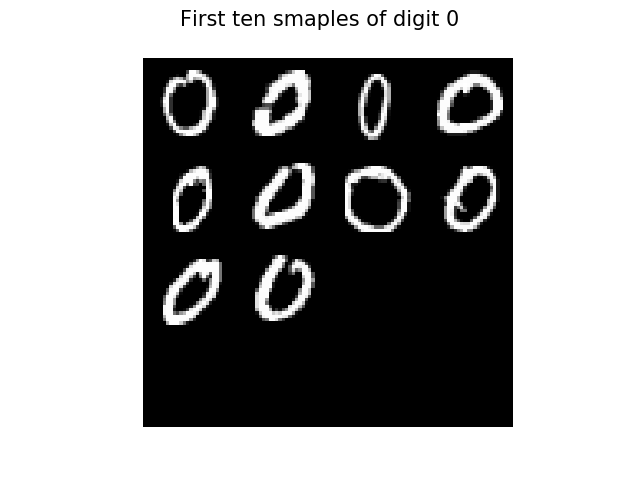
\includegraphics[trim=3cm 0 0 0, scale=0.4]{images/task1_1_imgs_class0.png}
    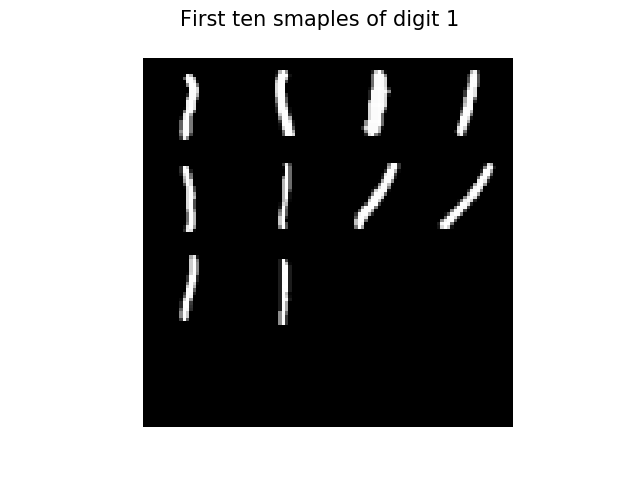
\includegraphics[trim=3cm 0 0 0, scale=0.4]{images/task1_1_imgs_class1.png}
    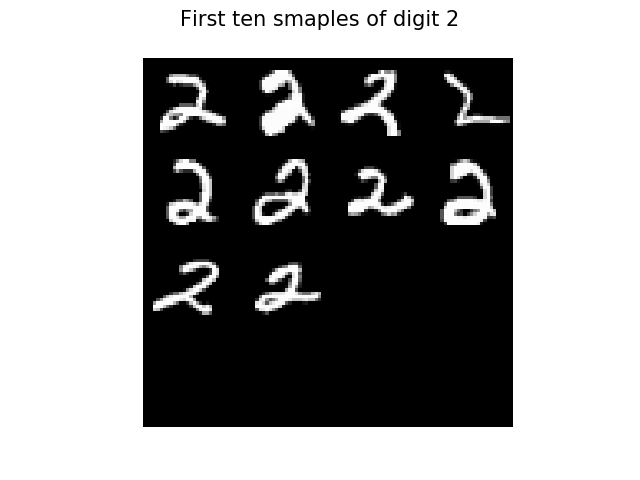
\includegraphics[trim=3cm 0 3cm 0, scale=0.4]{images/task1_1_imgs_class2.png}
\end{center}
    \\
\begin{center}
    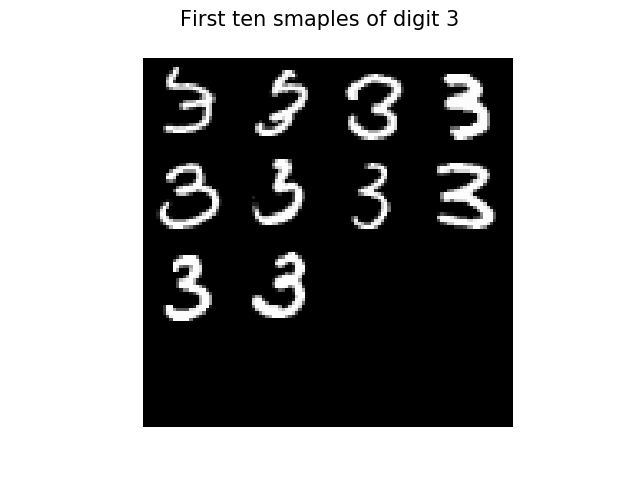
\includegraphics[trim=3cm 0 0 0, scale=0.4]{images/task1_1_imgs_class3.png}
    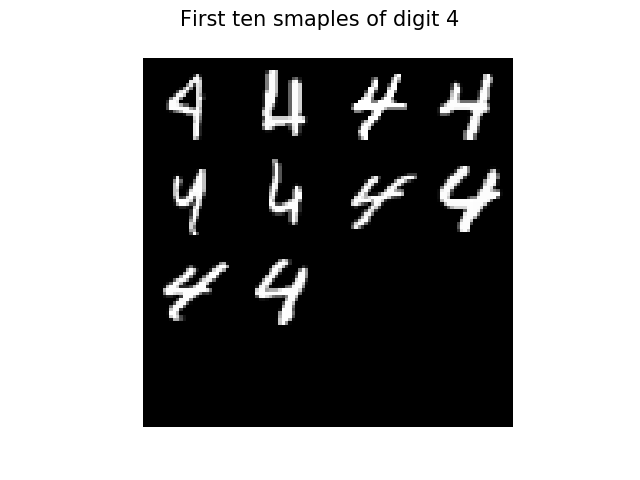
\includegraphics[trim=3cm 0 0 0, scale=0.4]{images/task1_1_imgs_class4.png}
    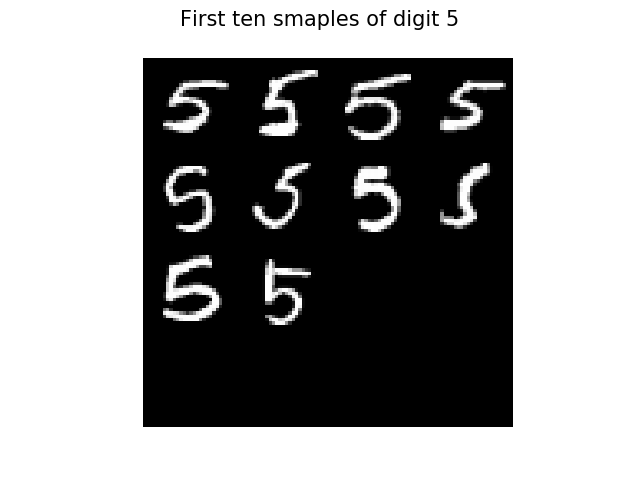
\includegraphics[trim=3cm 0 3cm 0, scale=0.4]{images/task1_1_imgs_class5.png}
\end{center}
    \\
\begin{center}
    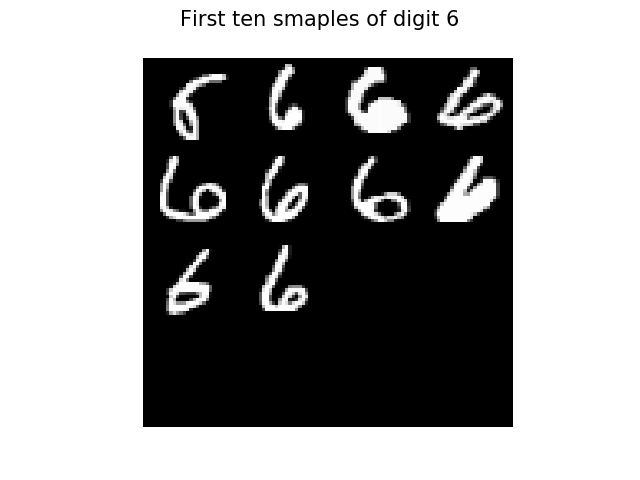
\includegraphics[trim=3cm 0 0 0, scale=0.4]{images/task1_1_imgs_class6.png}
    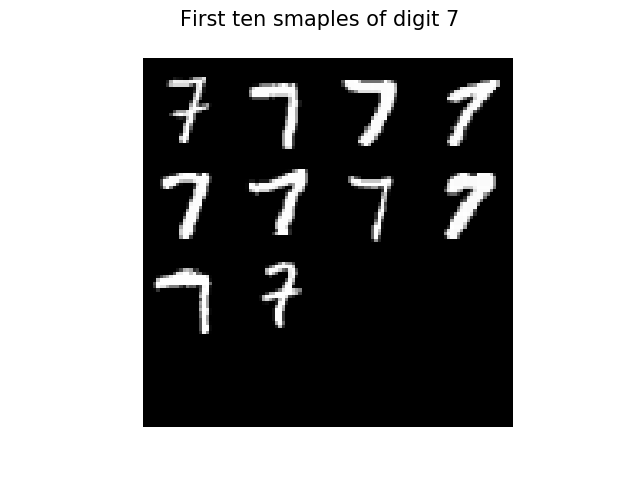
\includegraphics[trim=3cm 0 0 0, scale=0.4]{images/task1_1_imgs_class7.png}
    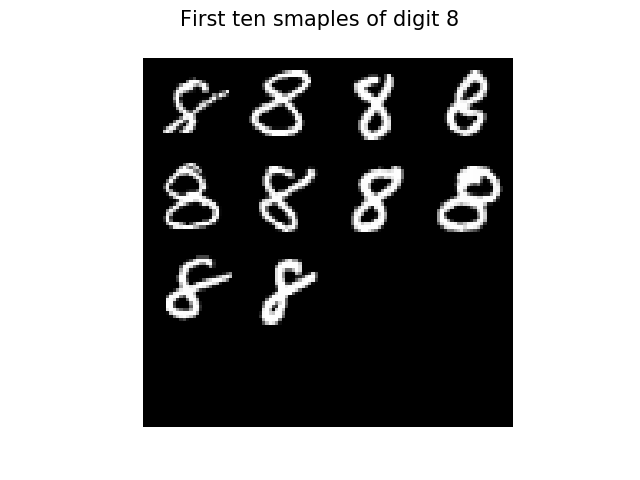
\includegraphics[trim=3cm 0 3cm 0, scale=0.4]{images/task1_1_imgs_class8.png}
\end{center}
    \\
\begin{center}
    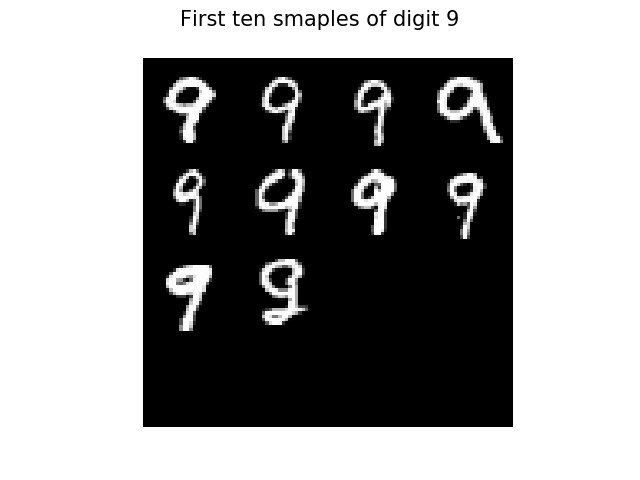
\includegraphics[trim=0 0 0 0, scale=0.4]{images/task1_1_imgs_class9.png}
\end{center}

\newpage

\subsection*{Task 1.2}

\begin{center}
    
\includegraphics[trim=0 0 0 0, scale=0.55]{images/task1_2_imgs.png}
\end{center}

\subsection*{Task 1.3}

\begin{center}
    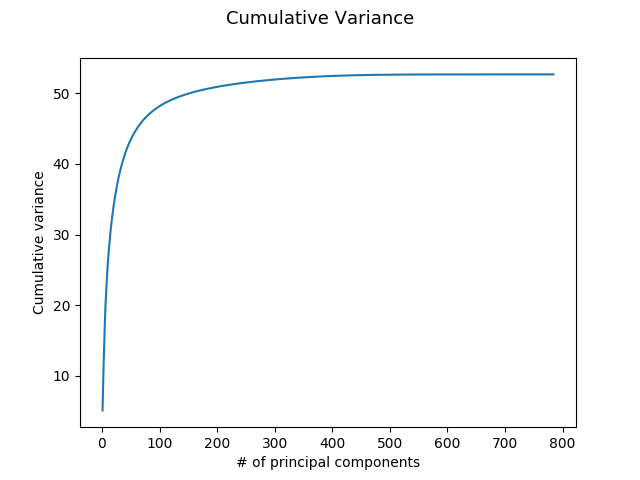
\includegraphics[trim=0 0 0 0, scale=0.5]{images/task1_3_graph.png}
\end{center}

\subsection*{Task 1.4}

\begin{center}
    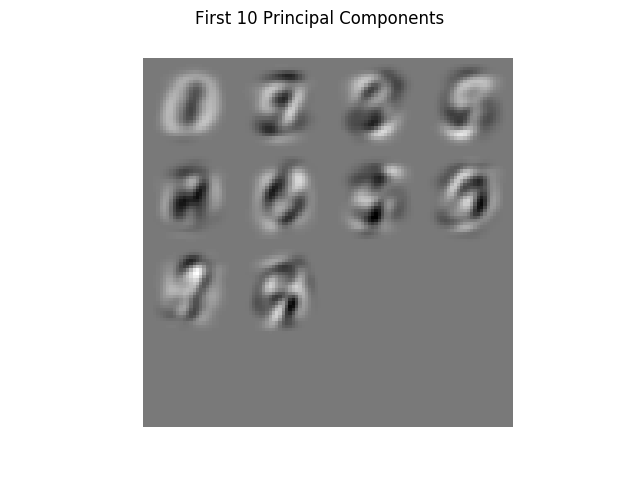
\includegraphics[trim=0 0 0 0, scale=0.55]{images/task1_4_imgs.png}
\end{center}


\subsection*{Task 1.5}

\subsubsection*{SSE over iterations for each K}

\begin{center}
    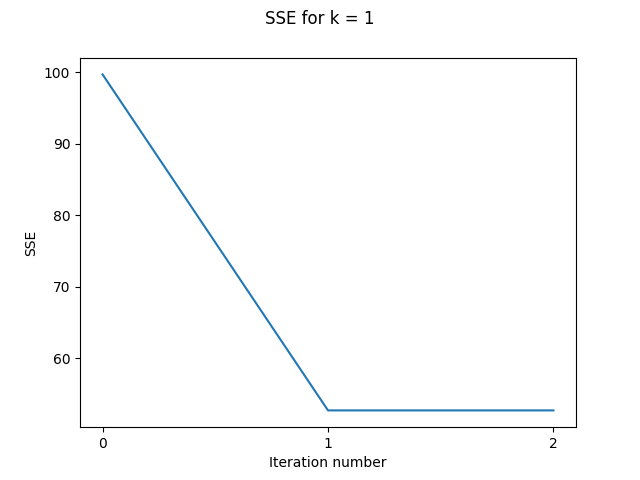
\includegraphics[scale=0.4]{images/task1_5_graph_1.png}
    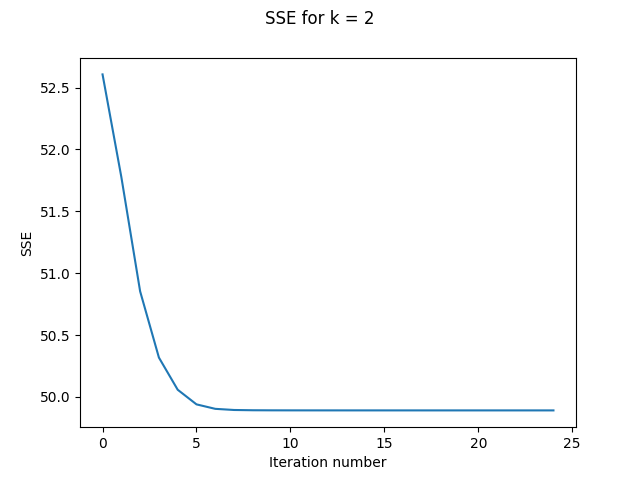
\includegraphics[scale=0.4]{images/task1_5_graph_2.png}
\end{center}
\vspace{0.2cm}
\begin{center}
    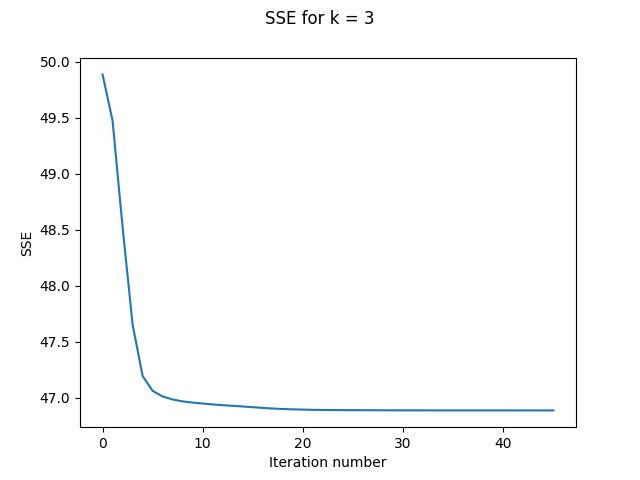
\includegraphics[scale=0.4]{images/task1_5_graph_3.png}
    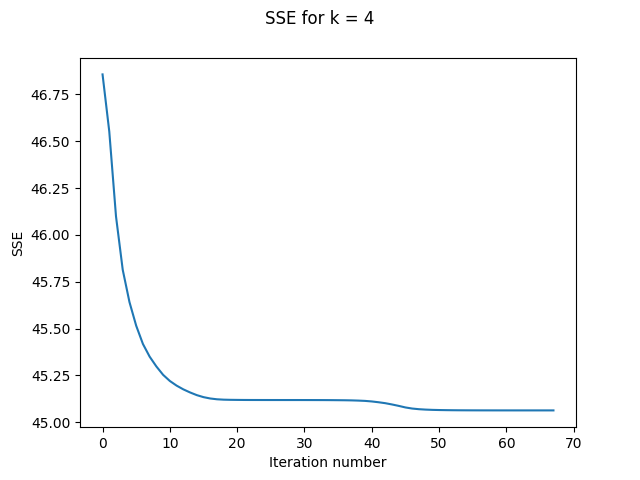
\includegraphics[scale=0.4]{images/task1_5_graph_4.png}
\end{center}
\vspace{0.2cm}
\begin{center}
    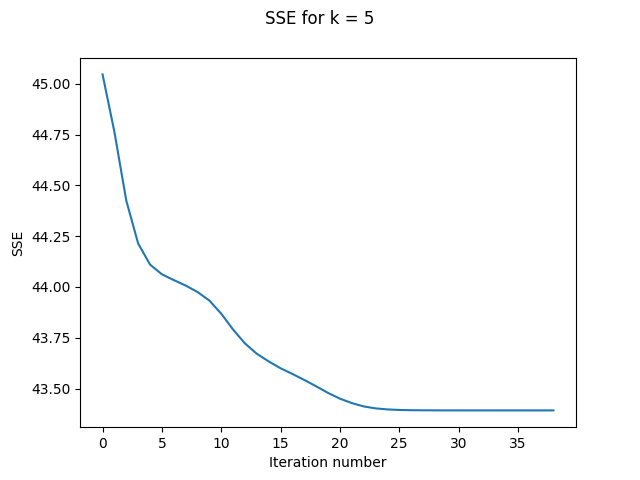
\includegraphics[scale=0.4]{images/task1_5_graph_5.png}
    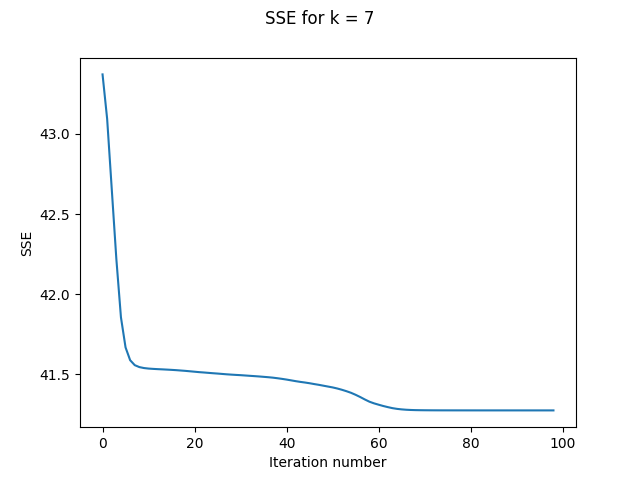
\includegraphics[scale=0.4]{images/task1_5_graph_7.png}
\end{center}
\vspace{0.2cm}
\begin{center}
    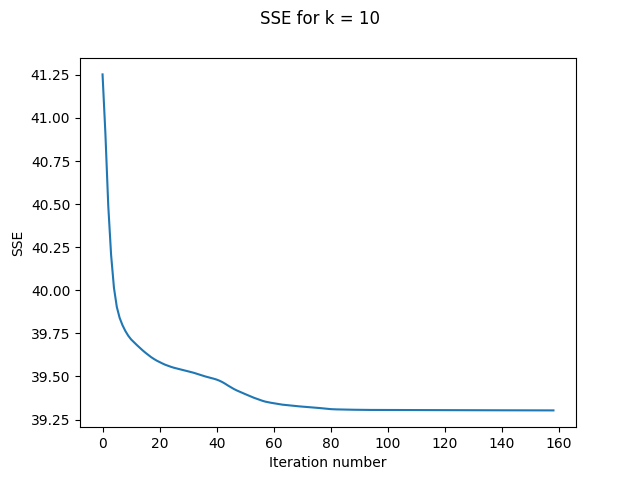
\includegraphics[scale=0.4]{images/task1_5_graph_10.png}
    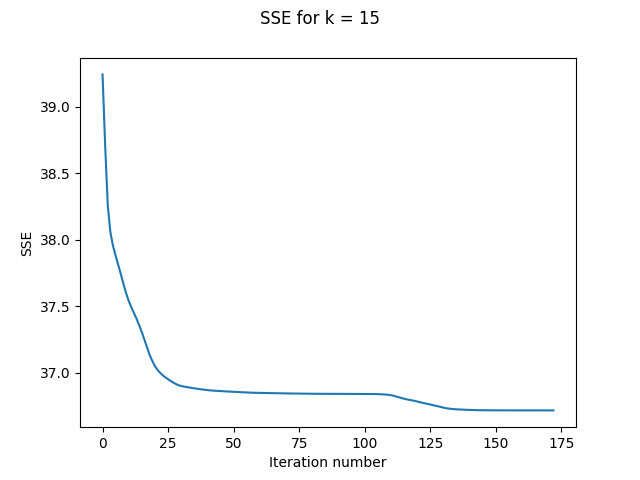
\includegraphics[scale=0.4]{images/task1_5_graph_15.png}
\end{center}

\begin{center}
    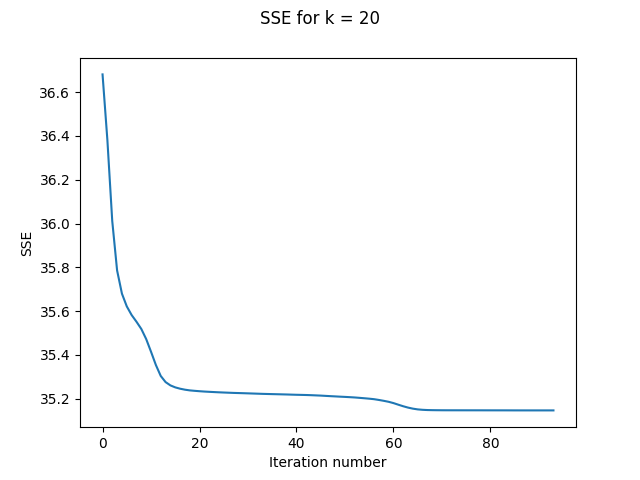
\includegraphics[scale=0.4]{images/task1_5_graph_20.png}
\end{center}

\subsubsection*{Runtimes for each K}
% Elapsed time in clustering for k = 1: 0.42484998703 secs
% Elapsed time in clustering for k = 2: 6.31980085373 secs
% Elapsed time in clustering for k = 3: 15.1873910427 secs
% Elapsed time in clustering for k = 4: 17.5111539364 secs
% Elapsed time in clustering for k = 5: 9.24557995796 secs
% Elapsed time in clustering for k = 7: 25.3608300686 secs
% Elapsed time in clustering for k = 10: 36.5944530964 secs
% Elapsed time in clustering for k = 15: 42.4299778938 secs
% Elapsed time in clustering for k = 20: 27.1714558601 secs

\begin{tabular}{ |c|c|c|c|c|c| } 
 \hline
 K & 1 & 2 & 3 & 4 & 5 \\ 
 \hline
 Runtime (s) & 0.42485 & 6.31980 & 15.18739 & 17.51115 & 9.24558 \\
 \hline
\end{tabular}


\begin{tabular}{ |c|c|c|c|c| } 
 \hline
 K & 7 & 10 & 15 & 20 \\ 
 \hline
 Runtime (s) & 25.36083 & 36.59445 & 42.42998 & 27.17146 \\
 \hline
\end{tabular}


\newpage
\subsection*{Task 1.6}

\begin{center}

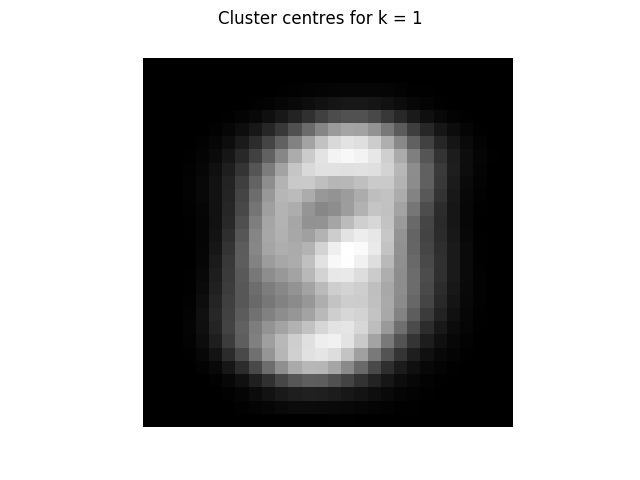
\includegraphics[trim=3cm 0 0 0, scale=0.4]{images/task1_6_imgs_1.png}
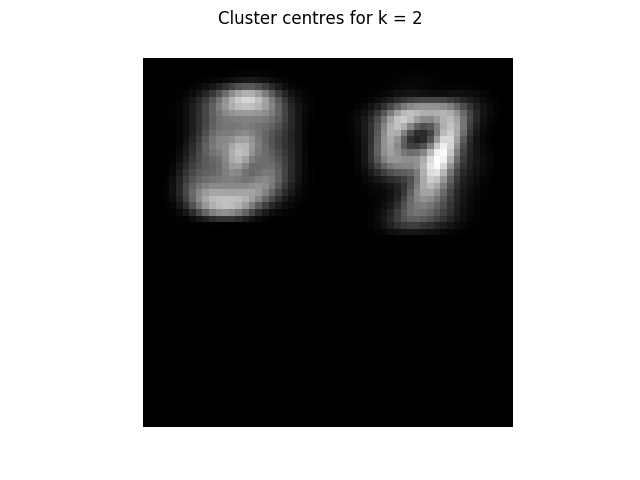
\includegraphics[trim=3cm 0 0 0, scale=0.4]{images/task1_6_imgs_2.png}
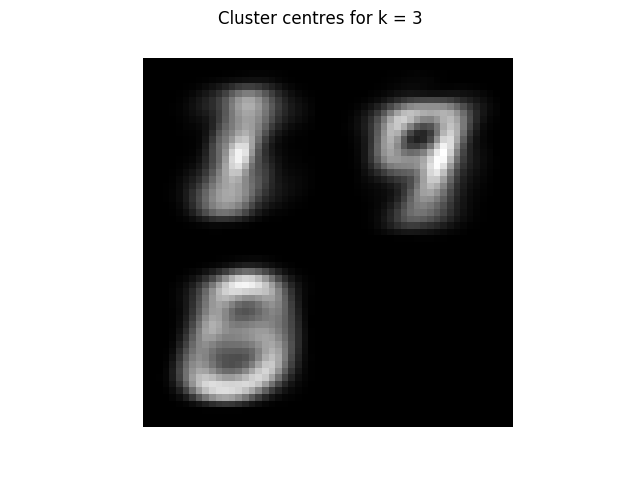
\includegraphics[trim=3cm 0 3cm 0, scale=0.4]{images/task1_6_imgs_3.png}
\\
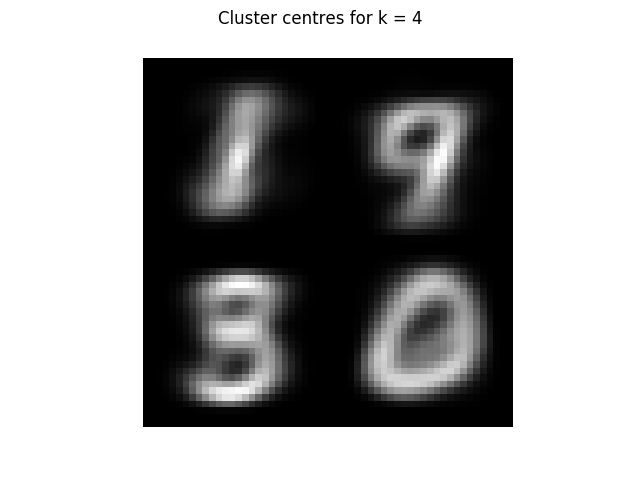
\includegraphics[trim=3cm 0 0 0, scale=0.4]{images/task1_6_imgs_4.png}
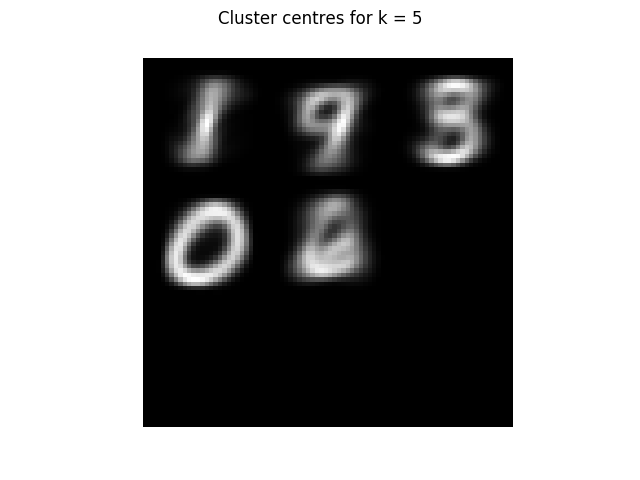
\includegraphics[trim=3cm 0 0 0, scale=0.4]{images/task1_6_imgs_5.png}
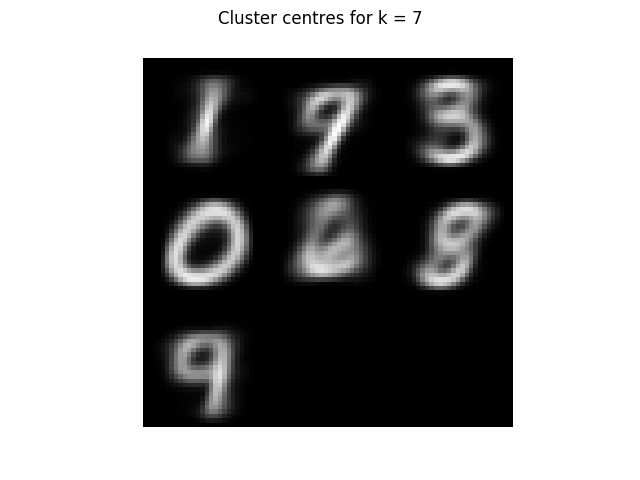
\includegraphics[trim=3cm 0 3cm 0, scale=0.4]{images/task1_6_imgs_7.png}
\\
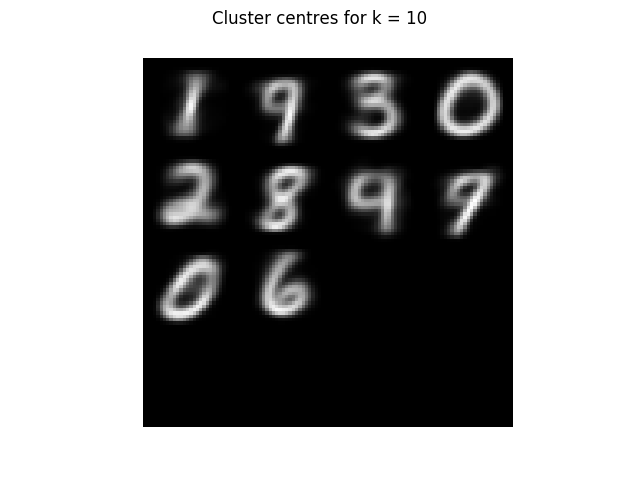
\includegraphics[trim=3cm 0 0 0, scale=0.4]{images/task1_6_imgs_10.png}
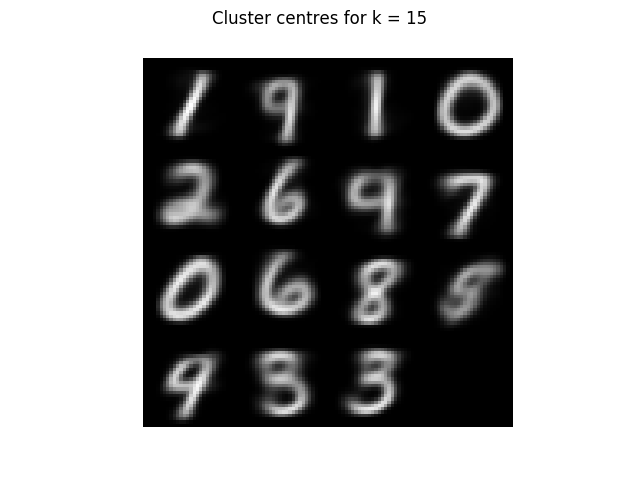
\includegraphics[trim=3cm 0 0 0, scale=0.4]{images/task1_6_imgs_15.png}
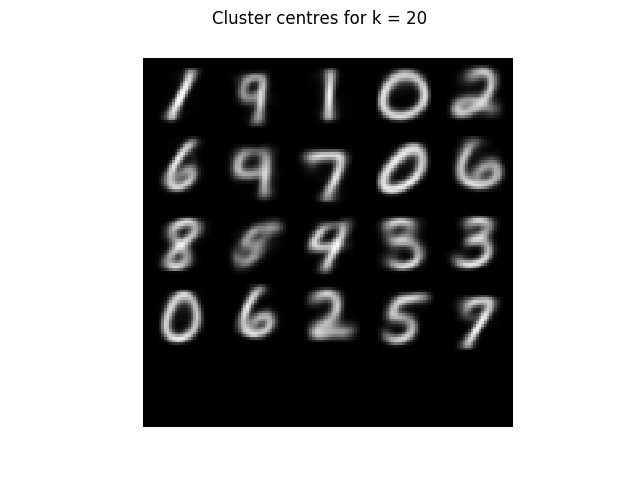
\includegraphics[trim=3cm 0 3cm 0, scale=0.4]{images/task1_6_imgs_20.png}

\end{center}

\newpage
\subsection*{Task 1.7}

\begin{center}
    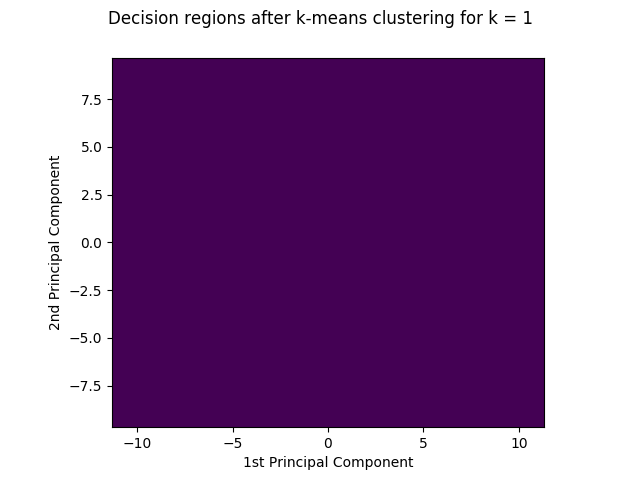
\includegraphics[trim=3cm 0 0 0, scale=0.5]{images/task1_7_1.png}
    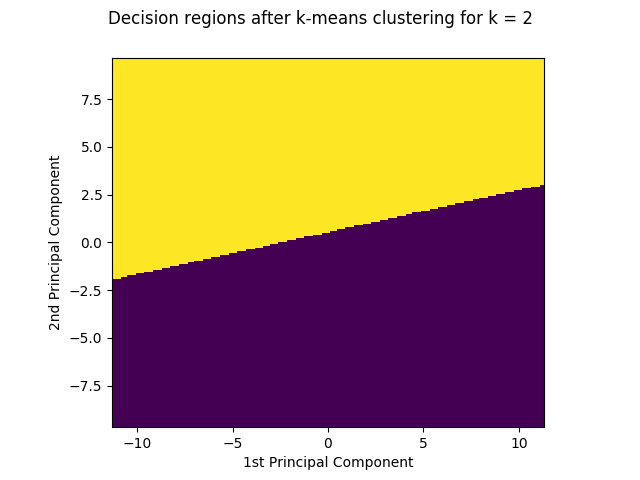
\includegraphics[trim=3cm 0 3cm 0, scale=0.5]{images/task1_7_2.png}
    \vspace{0.5cm}
    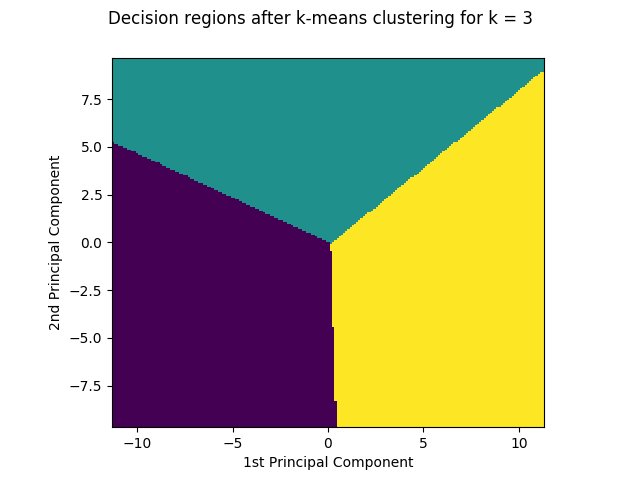
\includegraphics[trim=3cm 0 0 0, scale=0.5]{images/task1_7_3.png}
    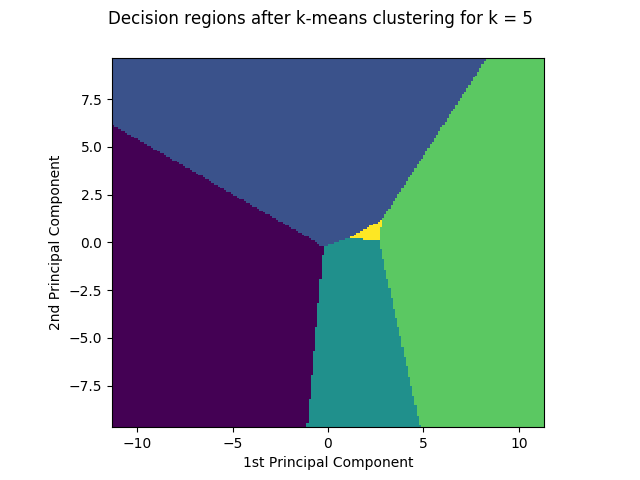
\includegraphics[trim=3cm 0 3cm 0, scale=0.5]{images/task1_7_5.png}
    \vspace{0.5cm}
    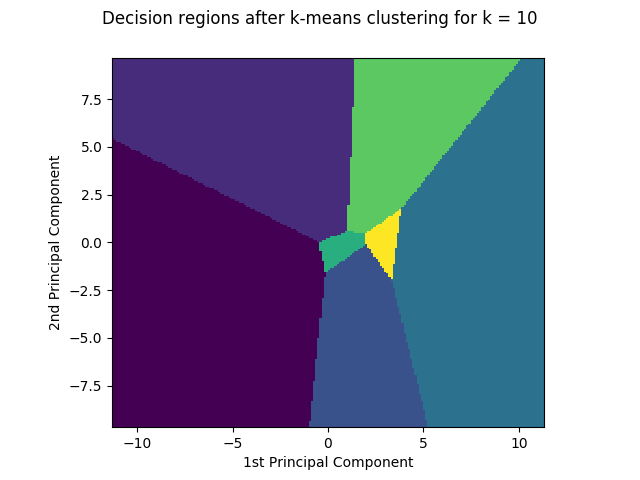
\includegraphics[scale=0.5]{images/task1_7_10.png}
\end{center}

\newpage
\subsubsection*{Methodology}
\renewcommand{\vec}[1]{\mathbf{#1}}

To plot these graphs we start by loading the previously calculated eigenvalues and eigenvectors of the data. From them, we extract the standard deviation ($\sigma$) for the first two principal components, that is, the square roots of the two largest eigenvalues. \\
After that, we load the mean vector of the dataset, and project it to the two-dimensional principal subspace, by multiplying it by the matrix containing the eigenvectors as columns. \\
The next step is to create a grid. However, first we need to determine the range of the plotting. To do that, we use the projected mean vector ($\mu$) to calculate the desired $\mu \pm 5\sigma$ range for each of the axes. In this interval we generate a linear space (\texttt{np.linspace()}) with 200 samples for each axis (value of \texttt{nbins}). These can then be combined by \texttt{np.meshgrid()} to obtain our grid of coordinates. \\
Now each of the points in that grid needs to be classified, but this grid is in a two-dimensional subspace and we want our classification to be done in the original vector space. To achieve this, we can 'unproject' the grid. \\
Each point in the two-dimensional subspace ($\vec{y}$) is obtained by projecting a corresponding point ($\vec{x}$) in the original vector space. This process is described by the formula (where $\vec{p}$ is the position vector, $\vec{y}$ is the projected data, $\vec{x}$ is the original data, and $\vec{V}$ is a matrix with the eigenvectors as columns):

\[
\vec{y} = \vec{V^T} \dot (\vec{x} - \vec{p}) \Leftrightarrow
\vec{x} = (\vec{V^T)^{-1}} \vec{y} + \vec{p}
\]
By first padding the grid elements with zeros to match the original dimensions and then applying the right-hand side of the equivalence we 'unproject' our grid. Finally, we can assign each point in the 'unprojected' grid to the closest cluster center obtaining our \texttt{Dmap}, which is used to plot the graphs above.

\newpage
\subsection*{Task 1.8}

For this small research project we were asked to investigate the impact of the initial cluster centres chosen in the performance of k-means clustering. The first step was the decision to work exclusively with $k = 10$ and use the previously suggested method (using the first ten samples of the dataset as initial centres) as our 'control subject'. Please note that each of these samples belongs to a different class.

From there, the experimentation was split into different branches:
\setlist{nosep}
\setlist[1]{noitemsep}
\setlist[2]{noitemsep}
\begin{enumerate}[]
    \item Options that would always be available
    \begin{enumerate}
        \item Randomly pick 10 samples, from any class, from the dataset
        \item Calculate the mean of the dataset and choose the 10 samples which are further     away from it
    \end{enumerate}
    \item Options that would only be possible with already tagged data (supervised learning - and so not very useful in a real world context)
        \begin{enumerate}
        \item Randomly pick 10 samples, one from each class, from the dataset
        \item Use the mean of each class as the initial cluster centres
    \end{enumerate}
\end{enumerate}

Please find the results obtained in the last page.

\subsubsection*{Conclusions}

The main observation about these results is that choosing initial centres away from the mean seems to be more efficient in the sense that the it results in a significantly lower number of iterations. The final sum squared error is marginally higher but there do not seem to be many fluctuations of that parameter. Complete randomness is the next best approach. \par
Additionally, we can also observe by the shape of the graphs that the error decreases much quicker when the initial centres are the furthest from the mean. This means that if we set a looser early termination condition we could safely cut the number of iterations down to about one fourth or less (in our example). \par
Finally, it also becomes apparent that having more information about the data (in this case the actual labels) does not seem to help us do a better job in estimating good initial cluster centres. \par
Overall, the main hypothesis is that the furthest the initial centres are from the mean of each class, the faster the process seems to converge. However to confidently claim this hypothesis would require further and more advanced testing.

\\

\subsubsection*{Results}

\begin{center}
\begin{tabular}{ |c|c|c|c|c|c| } 
 \hline
 Method & 'Control' & 1. (a) & 1. (b) & 2. (a) & 2. (b) \\ 
 \hline
 Number of iterations & 78 & 74 & 43 & 52 & 112 \\
 \hline
 Final error & 39.15347 & 39.15347 & 39.35176 & 39.32280 & 39.29411 \\
 \hline
\end{tabular}
\end{center}

\newpage
\begin{center}
    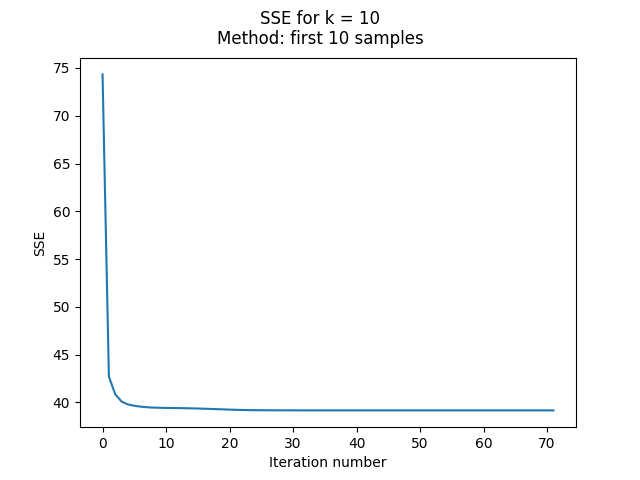
\includegraphics[trim=3cm 0 0 0, scale=0.5]{images/task1_8_0.png}
    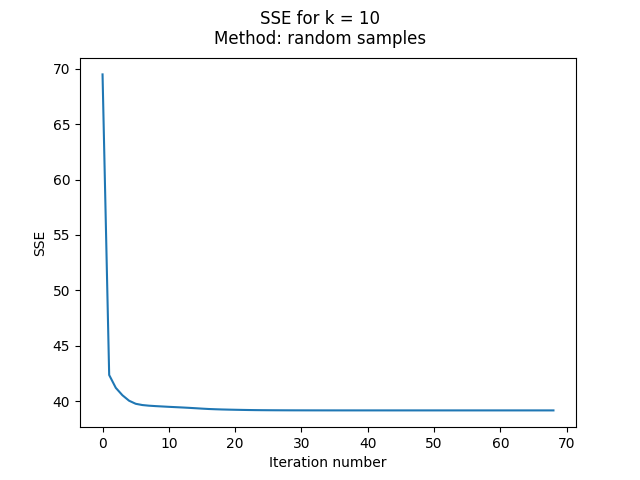
\includegraphics[trim=0 0 3cm 0, scale=0.5]{images/task1_8_1.png}
    \vspace{0.5cm}
    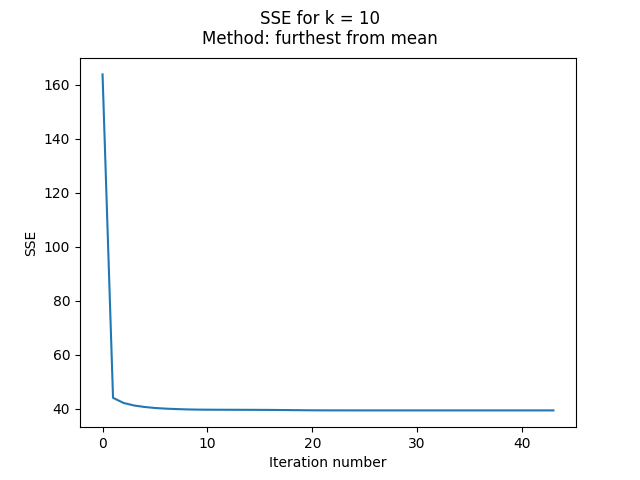
\includegraphics[trim=3cm 0 0 0, scale=0.5]{images/task1_8_2.png}
    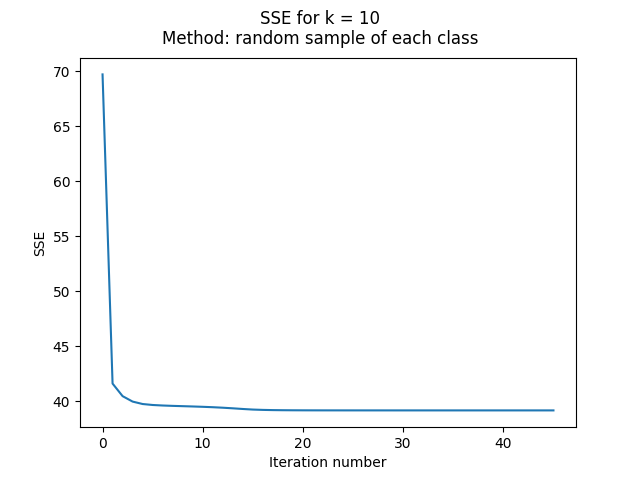
\includegraphics[trim=0 0 3cm 0, scale=0.5]{images/task1_8_3.png}
    \vspace{0.5cm}
    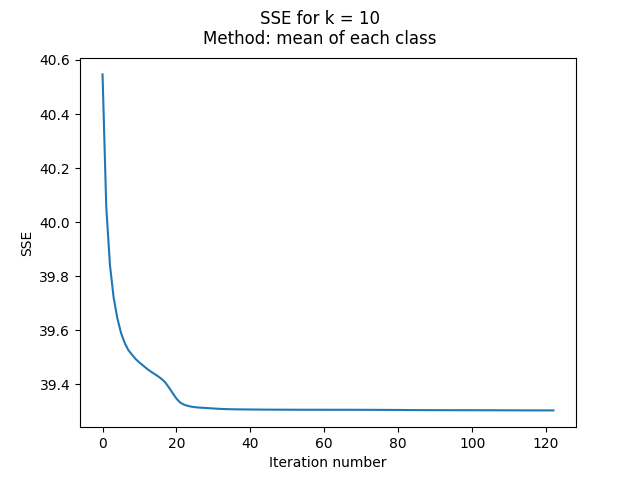
\includegraphics[scale=0.5]{images/task1_8_4.png}
\end{center}

%-------------- End of task 1 % ------------

\end{document}
